\begin{frame}{Testing}
    \begin{block}{What is tested?}
        \begin{itemize}
            \item Range
            \item Accuracy (Packetloss)
            \item Simple Antenna
            \item Speed
        \end{itemize}       
    \end{block} 
\end{frame}

\begin{frame}{Test 1: Antenna, Accuracy and Range.}
    \begin{block}{Variables:}
        \begin{itemize}
            \item Range
            \item Antenna on reciver (0 cm, 12 cm, 17.3 cm)
            \item Antenna on transmitter (0 cm, 12 cm, 17.3 cm)
        \end{itemize}
    \end{block}
    

    \begin{minipage}[0.3\textheight]{\textwidth}
        \begin{columns}[T]
            \begin{column}{0.3\textwidth}
                \begin{figure}
                    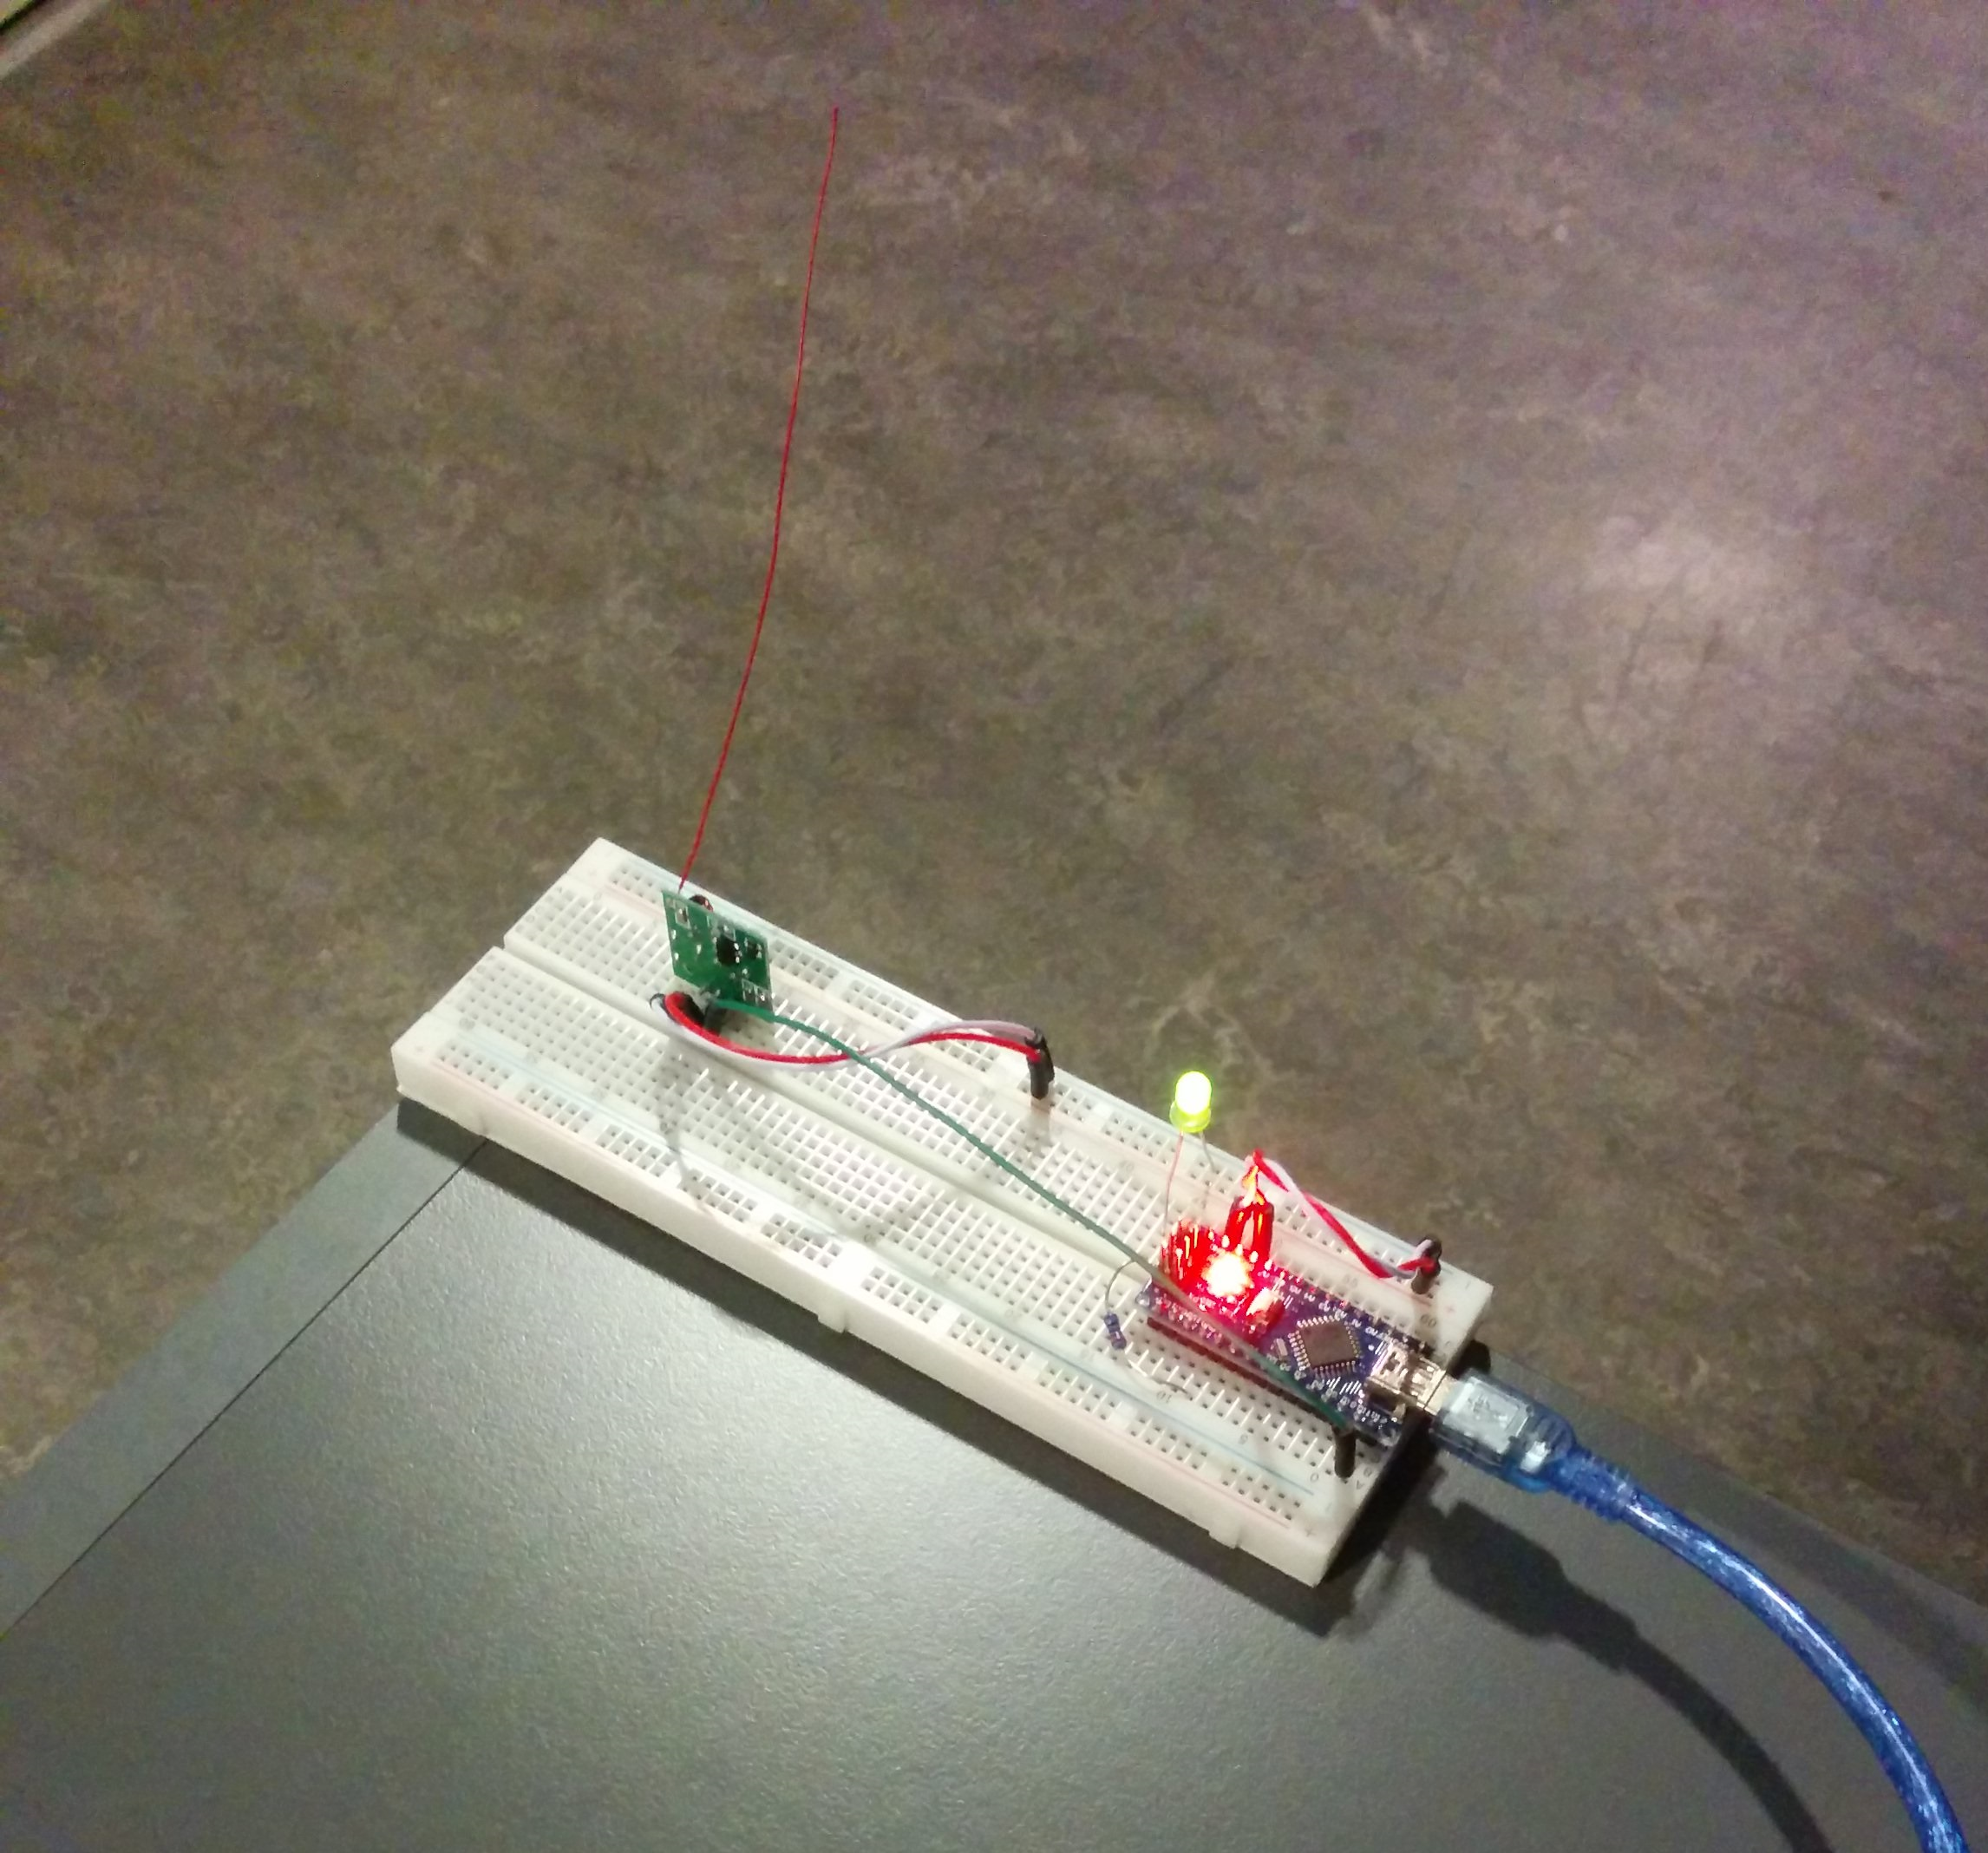
\includegraphics[height=0.45\textheight,keepaspectratio]{figures/Test_Pic.jpg}
                    \caption*{Transmitter used in test}
                \end{figure}
            \end{column}

            \begin{column}{0.6\textwidth}
                \hspace{10 pt}
                \begin{figure}
                    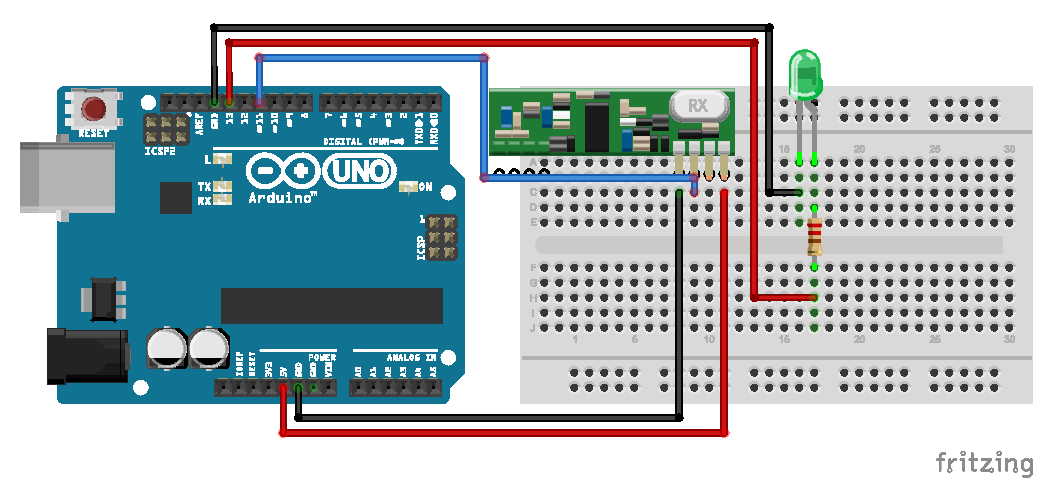
\includegraphics[height=0.35\textheight,keepaspectratio]{figures/reciver_diagram.pdf}
                    \caption*{Transmitter used in test}
                \end{figure}
            \end{column}
        \end{columns}
    \end{minipage}

\end{frame}

\begin{frame}{Test 1: Antenna, Accuracy and Range.}
    \begin{block}{Results:}
        \begin{itemize}
            \item Use a \textcolor{ReneOrange}{17.3 cm antenna} $(\frac{c}{433 MHz} * \frac{1}{4} = 17.3 cm)$
            \item Expect\textcolor{ReneOrange}{$~1 \%$ packet loss} 
            \item Some variables not accounted for:
            \begin{itemize}
                \item Objects in line of sight
                \item Location of test (basement)
                \item Others using the 433 MHz frequency
            \end{itemize}
        \end{itemize}
    \end{block}
    
    \begin{figure}
        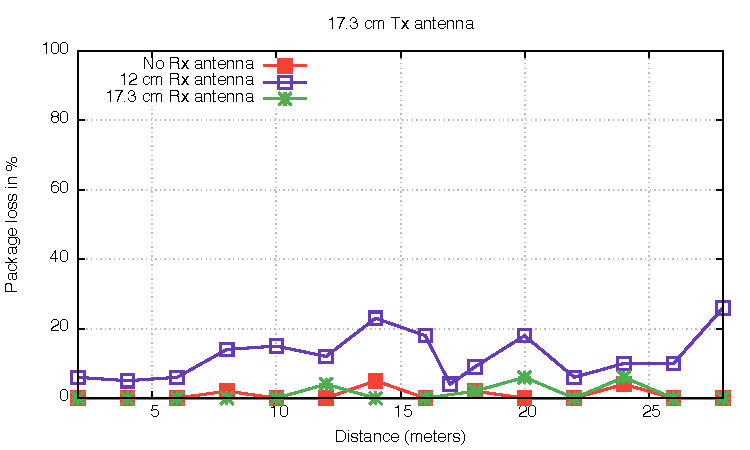
\includegraphics[height=0.4\textheight,keepaspectratio]{figures/17cm_ant.pdf}
    \end{figure}
\end{frame}

\begin{frame}{Test 2: Speed}
    What is the speed of the RF-Modules when using Radiohead?
    \begin{block}{Setup:}
        \begin{itemize}
            \item Send package; Wait 100 ms; Repeat with packagesize + 1 upto 60.
        \end{itemize}
    \end{block}

    \begin{block}{Result:}<2>
        \begin{itemize}
            \item $time(n)=6 * x + 65$, n is message length in bytes.
        \end{itemize}
    \end{block}
    
    \begin{figure}
        \includegraphics<2>[height=0.4\textheight,keepaspectratio]{figures/time_length.pdf}
    \end{figure}
\end{frame}

\begin{frame}{How to organize the network?}
    \begin{itemize}
        \item What is the best way to assign the timeslots within each frame?
        \item What is the worst case timeslot assignment when sending a message?
    \end{itemize}
    
    Devices:
       
    \vspace{10pt}
    \begin{center}
        \begin{tikzpicture}[->,>=stealth',shorten >=1pt,auto,node distance=3cm,
                        thick,main node/.style={circle,draw,font=\sffamily\Large\bfseries}]

          \node[main node] (1) {1};
          \node[main node] (2) [right of=1] {2};
          \node[main node] (3) [right of=2] {3};
          \node[main node] (4) [right of=3] {4};

          \path[every node/.style={font=\sffamily\small}]
            (1) edge node {} (2)
            (2) edge node {} (1)
            (3) edge node {} (2)
            (3) edge node {} (4)
            (4) edge node {} (3)
            (2) edge node {} (3);
        \end{tikzpicture}
    \end{center}
    
    Timeslot allocation:
    \\
    \vspace{10pt}
    \begin{center}
        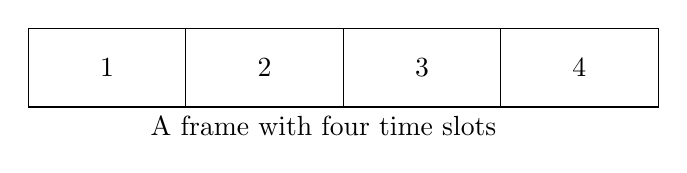
\begin{tikzpicture}[auto]
            \path[draw] (-5,0) -- (-5,1) -- (3,1) -- (3,0) -- (-5,0)
                        (-3,1) -- (-3,0)
                        (-1,1) -- (-1,0)
                        (1,1) -- (1,0)
                        (3,1) -- (3,0);
                        
            \node at (-4,0.5) {1};
            \node at (-2,0.5) {2};
            \node at (0,0.5) {3};
            \node at (2,0.5) {4};
                
            \path (1.5,0) -- node{A frame with four time slots} (-4,0);
        \end{tikzpicture}
    \end{center}
\end{frame}

\begin{frame}{How to organize the network?}
    \begin{itemize}
        \item What is the best way to assign the timeslots within each frame?
        \item What is the worst case timeslot assignment when sending a message?
    \end{itemize}
    \vspace{20pt}
    \begin{minipage}[0.3\textheight]{\textwidth}
        \begin{columns}[T]
            \begin{column}{0.5\textwidth}
                Devices:
                \begin{center}
                    \begin{tikzpicture}[->,>=stealth',shorten >=1pt,auto,node distance=2cm,
                                    thick,main node/.style={circle,draw,font=\sffamily\Large\bfseries}]

                      \node[main node] (1) {1};
                      \node[main node] (2) [right of=1] {2};
                      \node[main node] (3) [right of=2] {3};
                      \node[main node] (4) [above of=2] {4};
                      \node[main node] (5) [below of=2] {5};


                      \path[every node/.style={font=\sffamily\small}]
                        (1) edge node {} (2)
                        (2) edge node {} (1)

                        (3) edge node {} (2)
                        (2) edge node {} (3)

                        (5) edge node {} (2)
                        (2) edge node {} (5)

                        (4) edge node {} (2)
                        (2) edge node {} (4);
                    \end{tikzpicture}
                \end{center}
            \end{column}

            \begin{column}{0.5\textwidth}
                Timeslot allocation:
                \\
                \vspace{10pt}
                \begin{center}
                    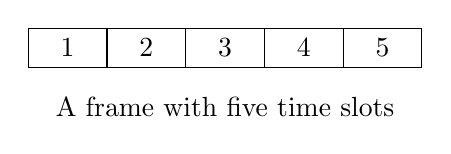
\begin{tikzpicture}[scale=0.50, node distance=3cm]
                        \path[draw] (-5,0) -- (-5,1) -- (5,1) -- (5,0) -- (-5,0)
                            (-3,1) -- (-3,0)
                            (-1,1) -- (-1,0)
                            (1,1) -- (1,0)
                            (3,1) -- (3,0);
                            
                        \node at (-4,0.5) {1};
                        \node at (-2,0.5) {2};
                        \node at (0,0.5) {3};
                        \node at (2,0.5) {4};
                        \node at (4,0.5) {5};
                            
                        \path (4.5,-1) -- node{A frame with five time slots} (-4.5,-1);        
                    \end{tikzpicture}
                \end{center}
            \end{column}
        \end{columns}
    \end{minipage}
\end{frame}
